\section{Experimental Evaluation}
\label{sec:experiments}

\subsection{Experimental Protocol}

\paragraph{Dataset} 
\label{sec:dataset}

The proposed training methods are evaluated on the PASCAL
VOC 2012 segmentation benchmark \citep{everingham2014pascal},
consisting of 20 foreground object classes and one background
class. The performance is measured in terms of pixel
intersection-over-union (IOU) averaged across the 21 classes. The
original PASCAL VOC 2012 dataset contains $1464$ (\textsl{train}),
$1449$ (\textsl{val}), and $1456$ (\textsl{test}) images for training,
validation, and test, respectively. In some experiments we also use
the extra annotations provided by \citet{hariharan2011semantic},
resulting in augmented sets of $10,582$ (\textsl{train\_aug}) and
$12,031$ (\textsl{trainval\_aug}) images. We have also experimented
with the large MS-COCO 2014 dataset \citep{lin2014microsoft}, which
contains $123,287$ images in its \textsl{trainval} set. The MS-COCO
2014 dataset has $80$ foreground object classes and one background
class and is also annotated at the pixel level.

Evaluation of our proposed methods is primarily conducted on the
PASCAL VOC 2012 \textsl{val} set but we also report results of selected
method variants submitted to the official PASCAL VOC 2012 server, which
evaluates results on the \textsl{test} set (whose annotations are not
released).

\paragraph{Training}

We employ our proposed training methods to learn the DCNN component of
the DeepLab-CRF model of \citet{chen2014semantic}. We start with the
Imagenet pretrained VGG-16 network of \citet{simonyan2014very},
modified as described in \citet{chen2014semantic}. In SGD training, we
use a mini-batch of 20 images and initial learning rate of $0.001$
($0.01$ for the final classifier layer), multiplying the learning rate
by 0.1 after a fixed number of iterations. We use momentum of $0.9$
and a weight decay of $0.0005$. Fine-tuning our network on PASCAL VOC
2012 takes about 12 hours on a NVIDIA Tesla K40 GPU. Our
implementation is based on the publicly available Caffe software
\citep{jia2014caffe}.

Similarly to \citet{chen2014semantic}, we decouple the DCNN and Dense
CRF training stages and learn the CRF parameters by cross validation
so as to maximize IOU segmentation accuracy in a held-out set of 100
Pascal \textsl{val} fully-annotated images. We use 10 mean-field
iterations for Dense CRF inference \citep{krahenbuhl2011efficient}.

\paragraph{Weak annotations}

In order to simulate the situations where only weak annotations are
available and to have fair comparisons (e.g., use the same images for
all settings), we generate the weak annotations from the pixel-level
annotations. The image-level labels are easily generated by
summarizing the pixel-level annotations, while the bounding box
annotations are produced by drawing rectangles tightly containing each
object instance (PASCAL VOC 2012 also provides instance-level
annotations) in the dataset.

\subsection{Model Training Using Fully Annotated Images}
\label{sec:test_pixel}

The performance of the DeepLab-CRF model trained with strong
pixel-level annotations sets a target upper bound which we try to
reach with the proposed algorithms for weakly- or semi-supervised
training. In reproducing the results of \citep{chen2014semantic} on
PASCAL VOC 2012 \textsl{val}, we have achieved a
\textsl{DeepLab-CRF(Strong)} IOU score of \textbf{63.9}\% (they
report a score of 63.7 in their Table~1a).

%% \begin{table}
%%   \centering
%%   \caption{{\bf{Pixel Annotations.}} Performance on the PASCAL VOC 2012 `val' set. First column, and second column show the number of strongly labeled images from PASCAL and MS-COCO. }
%%   \begin{tabular}{| c | c | c | c |}
%%     \hline
%%     \# PASCAL & \# MS-COCO & DeepLab & DeepLab-CRF \\
%%     \hline
%%     10,582 &   0     & 59.85 & 63.93  \\
%%     \hline
%%     10,582 & 123,287 & 64.51 & 67.98 \\
%%     \hline
%%     \end{tabular}
%%   \label{tb:pixel_annot}
%% \end{table}

\subsection{Model Training Using Bounding Box Weak Annotations}
\label{sec:test_bbox}

In this experiment we train the DeepLab-CRF model using the PASCAL VOC
2012 bounding box annotations, generated as described in
\secref{sec:dataset} above. We estimate the training set segmentations
in a pre-processing step using the \textsl{Bbox-Baseline} and
\textsl{Bbox-Seg} methods described in \secref{sec:train_bbox}.

We assume that we also have access to 100 fully-annotated PASCAL VOC
2012 \textsl{val} images which we have used to cross-validate the
value of the single \textsl{Bbox-Seg} parameter $\alpha$ (percentage
of the center bounding box area constrained to be foreground). We
varied $\alpha$ from 20\% to 80\%, finding that using $\alpha = 20\%$
maximizes the accuracy in terms of IOU in recovering the ground truth
foreground from the bounding box.

%% \begin{table}
%%   \centering
%%   \caption{\textsl{Bbox-Seg} parameter cross-validation.}
%%   \begin{tabular}{c | c c c c}
%%     $\alpha$ (\%)    &  80   &  60   &  40   &  20   \\
%%     \hline
%%     Pixel IOU (\%) & 65.6  & 68.8  & 71.8  & {\bf 72.6}
%%     \end{tabular}
%%   \label{tb:bbox_erosion}
%% \end{table}

The PASCAL VOC 2012 \textsl{val} performance achieved after training
the DeepLab-CRF model on the segmentations obtained by the
\textsl{Bbox-Baseline} and \textsl{Bbox-Seg} is reported in
\tabref{tb:bbox_annot}. We see that \textsl{Bbox-Seg} improves over
\textsl{Bbox-Baseline} by nearly 6\% but still lags by 5.5\% compared
to training with the strong pixel-level annotation.

\begin{table}
  \centering
  \caption{DeepLab-CRF VOC 2012 \textsl{val} IOU (\%) results
    using bounding box weak annotations \vs strong annotation in
    training.}
  \scalebox{0.9}{
  \begin{tabular}{c | c || c}
    Bbox-Baseline & Bbox-Seg & Strong \\
    \hline
    52.5          & 58.5     & 63.9
  \end{tabular}
  }
  \label{tb:bbox_annot}
\end{table}

%% \begin{table}
%%   \centering
%%   \caption{{\bf Bounding Box Annotations.} Performance on the PASCAL VOC 2012 `val' set. DeepLab and DeeLab-CRF are trained with the segmentation generated by Bbox-Baseline or Bbox-DenseCRF.}
%%   \begin{tabular}{| l | c | c |}
%%     \hline
%%      & DeepLab & DeepLab-CRF \\
%%     \hline
%%     Bbox-Baseline & 47.72 & 52.52 \\ 
%%     \hline
%%     Bbox-DenseCRF & 53.68 & 58.45 \\
%%     \hline
%%     \end{tabular}
%%   \label{tb:bbox_annot}
%% \end{table}

\subsection{Model Training Using Weak Image-Level Labels}
\label{sec:test_image}

We proceed with evaluating our proposed methods in training the
DeepLab-CRF model using just image-level weak PASCAL VOC 2012
annotations, generated as described in \secref{sec:dataset} above. We
report the \textsl{val} performance of our two weakly-supervised EM
variants described in \secref{sec:train_image}. In the
\textsl{EM-Fixed} variant we use $c_f = 6$ and $c_b = 5$ as fixed
foreground and background biases. We found the results to be quite
sensitive to the difference $c_f-c_b$ but not very sensitive to their
absolute values. In the adaptive \textsl{EM-Adapt} variant we
constrain at least 40\% of the image area to be assigned to background
and at least 20\% of the image area to be assigned to foreground (as
specified by the weak label set). 

The PASCAL VOC 2012 \textsl{val} performance achieved after training
the DeepLab-CRF model with this weakly-supervised EM algorithm are
reported in \tabref{tb:weak_annot}. This table also contains results
obtained by the previous MIL-based methods \textsl{MIL1}
\citep{pathak2014fully} and \textsl{MIL2}, \textsl{MIL2-ILP}
\citep{pinheiro2014weakly}. Note that the numbers are not directly
comparable because \citet{pathak2014fully} evaluates on the VOC 2011
\textsl{val} and \citet{pinheiro2014weakly} train the parameters of
their CNN models on the Imagenet dataset. 

We observe that \textsl{EM-Fixed} performs poorly on this challenging
task, at the same level as the previous \textsl{MIL1} and \textsl{MIL2}
methods. Similarly to them, we observed that the \textsl{EM-Fixed}
model had particularly difficulty in balancing the scores of the
foreground and background classes, often producing all-background
segmentations. The \textsl{MIL2-ILP} method partially alleviates this
problem by departing from the pure MIL formulation, also incorporating
image-level classification scores during training. Our
\textsl{EM-Adapt} method performed considerably better by explicitly
enforcing both background and foreground labels to emerge in the
estimation process. However, its performance at 38.2\% significantly
lags the target 63.9\% goal of the strongly-supervised model trained
on pixel-level annotations.

\begin{table}
  \centering
  \caption{Our DeepLab-CRF VOC \textsl{val} IOU (\%) results with
    image-level weak annotations in training \vs previous methods.} 
  \scalebox{0.9}{
  \begin{tabular}{c | c | c || c | c}
    MIL1  & MIL2 & MIL2-ILP & EM-Fixed & EM-Adapt \\
    \hline
    20.5  & 17.8 & 32.6     & 20.8     & 38.2
  \end{tabular}
  }
  \label{tb:weak_annot}
\end{table}


%% \begin{table}
%%   \centering
%%   \caption{{\bf Comparison with state-of-art methods on val set.}}
%%   \begin{tabular}{l|c}
%%     {\bf Method} & pixel IOU (\%) \\
%%     \hline \hline
%%     Idiap-base   & 17.8 \\
%%     DeepLab-Weak & 20.3 \\
%%     \hline \hline
%%     Idiap-base+ILP  & 32.6 \\
%%     DeepLab-Adaweak & 34.2 \\
%%     \hline \hline
%%     Idiap-base+ILP+sppxl & 36.6 \\
%%     DeepLab-CRF-Adaweak  & 38.2 \\
%%     \hline \hline
%%     Idiap-base+ILP+seg       & 42.0 \\
%%     DeepLab-CRF-StrongWeak   & 61.9 \\
%%   \end{tabular}
%%   \label{tab:weak_state_of_art_val}
%% \end{table}


\subsection{Semi-Supervised Model Training Using Both Fully and Weakly Annotated Images}
\label{sec:test_semi}

We next examine to what extent weak image-level annotations can
complement strong pixel-level annotations in training the DeepLab-CRF
model, using the semi-supervised learning methods of
\secref{sec:train_semi}. In this \textsl{Semi} setting we employ the
strong annotations of a subset of PASCAL VOC 2012 \textsl{train} set
and use just the weak image-level labels from another non-overlapping
subset of the \textsl{train\_aug} set. We perform segmentation
inference for the images that only have image-level labels by means of
\textsl{EM-Fixed}. In \tabref{tab:strong_weak_annot} we report the 
results obtained by varying the sizes of the strong and weak
annotation sets, also including for comparison the results of pure
weakly-supervised and strongly-supervised learning.

We observe that including even a few hundreds of strongly annotated
images in the semi-supervised setting significantly improves the 
performance compared to the pure weakly-supervised baseline. We also
observe that using just 1,464 strongly annotated images (13.8\% of the
\textsl{train\_aug} set) along with the remaining weakly annotated
images suffices to reach performance 61.9\%, only 2\% lower than the
result obtained by pure strongly-supervised training on all 10,582
\textsl{train\_aug} images. Note that only using the 1,464 strongly
annotated images in the \textsl{train} set and no weakly annotated
images performs significantly worse at 57.6\%, demonstrating the
significant benefits of the semi-supervised setting.

\begin{table}[t]
  \centering
  \caption{DeepLab-CRF VOC 2012 \textsl{val} IOU (\%) performance
    using both strong pixel-level and weak image-level annotations.}
  \scalebox{0.8}{
  \begin{tabular}{|c|c|c|c|}
    \hline
    \#Strong & \#Weak  & DeepLab-CRF  & Scenario\\
    \hline
    0        &  10,582 & 20.8         & Weak-EM-Fixed \\
    0        &  10,582 & 38.2         & Weak-EM-Adapt \\
    \hline\hline
    200      &  10,382 & 47.6         & \multirow{4}{*}{Semi} \\
    500      &  10,082 & 56.9   &\\
    750      &  9,832  & 58.8   &\\
    1,000    &  9,582  & 60.5   &\\
    \hline
    1,464    &  5,000  & 60.5         & \multirow{2}{*}{Semi} \\
    1,464    &  9,118  & 61.9   &\\
    \hline\hline
    1,464    &  0      & 57.6         & \multirow{2}{*}{Strong} \\
    10,582   &  0      & 63.9   &\\
    \hline
  \end{tabular}  
  }
  \label{tab:strong_weak_annot}
\end{table}


%% \begin{table}[t]
%%   \centering
%%   \caption{{\bf Pixel+Image Annotations.} }
%%   \scalebox{0.8}{
%%   %\addtolength{\tabcolsep}{-2.0pt}
%%   \begin{tabular}{|c|c|c|c|}
%%     \hline
%%     {\bf Weak} & {\bf Strong} & \multirow{2}{*}{DeepLab} & \multirow{2}{*}{DeepLab-CRF}\\
%%     \cline{1-2}
%%     \# PASCAL & \# PASCAL & & \\
%%     \hline
%%     10,582   &    0    & 20.25  & 20.77   \\
%%     \hline
%%     10,582   &    0    & 34.22* & 38.23*  \\
%%     \hline
%%     10,382   &  200    & 44.05  & 47.57   \\
%%     \hline
%%     10,082   &  500    & 52.52  & 56.89   \\
%%     \hline
%%     9,832    &  750    & 55.04  & 58.82   \\
%%     \hline
%%     9,582    &  1,000  & 56.79  & 60.48   \\
%%     \hline
%%       0      &  1,464  & 54.77  & 57.62   \\
%%     \hline
%%     5,000    &  1,464  & 57.02  & 60.48   \\
%%     \hline
%%     9,118    &  1,464  & {\bf 58.30}  & {\bf 61.90}   \\
%%     \hline
%%   \end{tabular}  
%%   }
%%   \label{tab:strong_weak_annot}
%% \end{table}


\subsection{Exploiting Annotations Across Datasets}
\label{sec:cross_dataset}

Finally, we present experiments leveraging the 81-label MS-COCO
dataset as an additional source of data in learning the DeepLab model
for the 21-label PASCAL VOC 2012 segmentation task. We consider
three scenarios:
\begin{itemize}
\item \textsl{Strong-Cross-Pretrain}: Pre-train DeepLab on MS-COCO,
  then replace the top-level classifiers weights and fine-tune on
  Pascal VOC 2012, using strong labels in both datasets.
\item \textsl{Strong-Cross-Joint}: Jointly train DeepLab on Pascal VOC
  2012 and MS-COCO, sharing the top-level classifier weights for the
  common classes, using strong labels in both datasets.
\item \textsl{Semi-Cross-Joint}: Jointly train DeepLab on Pascal VOC
  2012 and MS-COCO, sharing the top-level classifier weights for the
  common classes, using the strong labels from PASCAL and varying the
  number of strong and weak labels from MS-COCO.
\end{itemize}
In all cases we use strong annotations for all 10,582
\textsl{train\_aug} PASCAL images.

We report our results on the PASCAL VOC 2012 \textsl{val} in
\tabref{tab:cross_data}, also including for comparison our best
PASCAL-only 63.9\% result exploiting all 10,582 strong annotations as
a baseline. When we employ the weak MS-COCO annotations
(\textsl{Weak-EM-Fixed}) we obtain 64.4\% IOU, a marginal 0.5\%
improvement over the PASCAL-only baseline. Using strong labels from
5,000 MS-COCO images (4.0\% of the MS-COCO dataset) and weak labels
from the remaining MS-COCO images in the \textsl{Semi-Cross-Joint}
semi-supervised scenario yields 66.5\%, a significant 2.6\% boost over
the baseline. This \textsl{Semi-Cross-Joint} result is also 1.6\%
better than the 64.9\% performance obtained using only the 5,000
strong and no weak annotations from MS-COCO. As expected, our best
results are obtained by using all 123,287 strong MS-COCO
annotations. Both \textsl{Strong-Cross-Pretrain} and
\textsl{Strong-Cross-Joint} yield 68.0\% in this scenario. We observe
that cross-dataset augmentation significantly improves over the best
PASCAL-only result. Using only a small portion of pixel-level
annotations and a large portion of image-level annotations in the
semi-supervised setting suffices to reap most of this benefit.

\begin{table}[t]
  \centering
  \caption{DeepLab-CRF VOC 2012 \textsl{val} IOU (\%) performance
    using strong annotations for all 10,582 \textsl{train\_aug} PASCAL
    images and a varying number of strong and weak MS-COCO
    annotations.}
  \scalebox{0.8}{
  \begin{tabular}{|c|c|c|c|}
    \hline
    \#Strong & \#Weak  & DeepLab-CRF & Scenario \\
    \hline
    0        & 0       & 63.9        & PASCAL-only \\
    \hline\hline
    0        & 123,287 & 64.4        & Weak-EM-Fixed \\
    \hline\hline
    5,000    & 118,287 & 66.5        & Semi-Cross-Joint \\
    \hline\hline
    5,000    &  0      & 64.9        & Strong-Cross-Joint \\
    123,287  &  0      & 68.0        & Strong-Cross-Pretrain \\
    123,287  &  0      & 68.0        & Strong-Cross-Joint \\
    \hline
  \end{tabular}  
  }
  \label{tab:cross_data}
\end{table}

%% \begin{table}[t]
%%   \centering
%%   \caption{{\bf Pixel+Image Annotations with MS-COCO.} }
%%   \scalebox{0.77}{
%%   %\addtolength{\tabcolsep}{-2.0pt}
%%   \begin{tabular}{|c|c|c|c|c|}
%%     \hline
%%     {\bf Weak} & \multicolumn{2}{c|}{\bf Strong} & \multirow{2}{*}{DeepLab} & \multirow{2}{*}{DeepLab-CRF}\\
%%     \cline{1-3}
%%     \# MS-COCO & \# PASCAL & \# MS-COCO & & \\
%%     \hline
%%       0       & 10,582 & 0       & 59.85 & 63.93 \\
%%     \hline
%%       123,287 & 10,582 & 0       & 60.41 & 64.44 \\
%%     \hline
%%       0       & 10,582 & 5,000   & 61.34 & 64.91 \\
%%     \hline
%%       118,287 & 10,582 & 5,000   & ?     &  ?    \\
%%     \hline    
%%       0       & 10,582 & 123,287 & 64.51 & 67.98 \\
%%     \hline
%%   \end{tabular}  
%%   }
%%   \label{tab:strong_weak_annot_coco}
%% \end{table}


\subsection{Qualitative Segmentation Results} 
\label{sec:test_qualitative}

We provide in \figref{fig:ValResults} visual comparisons of the
results obtained by the DeepLab-CRF model learned with the proposed
training methods. The segmentation result of the model trained on only
weak labels (\textsl{Weak-EM-Adapt}) does capture the presence of
objects but is rather noisy. In the bounding box training scenario,
training with inferred segmentations (\textsl{Bbox-Seg}) significantly
improves the localization accuracy over \textsl{Bbox-Baseline}. Using
1,464 strong and 9,118 weak PASCAL annotations in the \textsl{Semi
  (1,464 strong)} experiment yields significantly better results. We
obtain the visually best segmentation results when using all available
strong annotations from both the PASCAL and MS-COCO datasets
(\textsl{Strong-Cross-Joint}).

\begin{figure*}[!htbp]
  \centering
  %\vspace{-1.cm}
  \scalebox{0.82} {
  \begin{tabular}{c c c c c c}
    %\addtolength{\tabcolsep}{-6.5pt}
    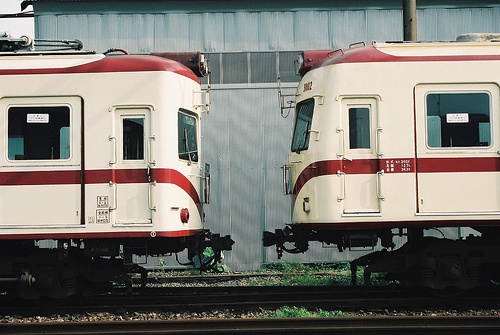
\includegraphics[height=0.11\linewidth]{fig/val_crf_vis/img/2007_000042.jpg} &
    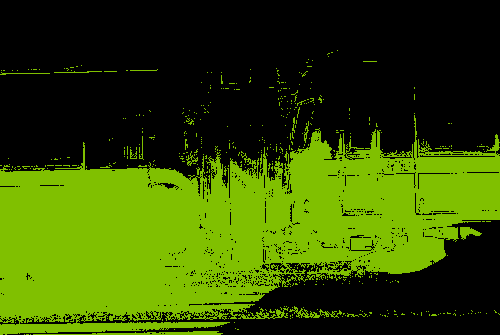
\includegraphics[height=0.11\linewidth]{fig/val_crf_vis/adaweak/2007_000042.png} &
    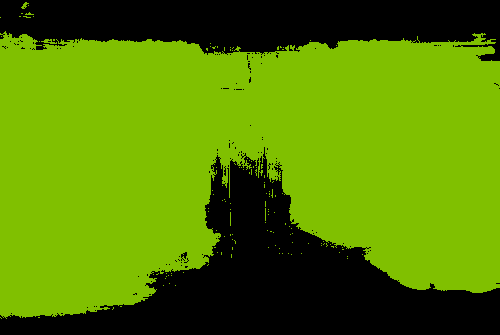
\includegraphics[height=0.11\linewidth]{fig/val_crf_vis/bbox/2007_000042.png} &
    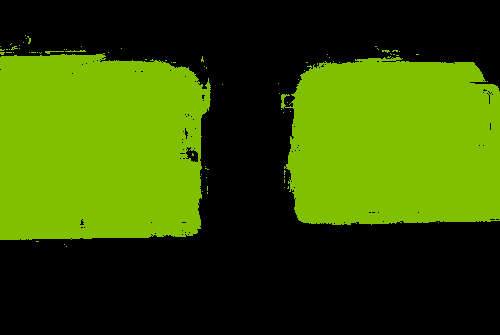
\includegraphics[height=0.11\linewidth]{fig/val_crf_vis/bbox_crf/2007_000042.png} &
    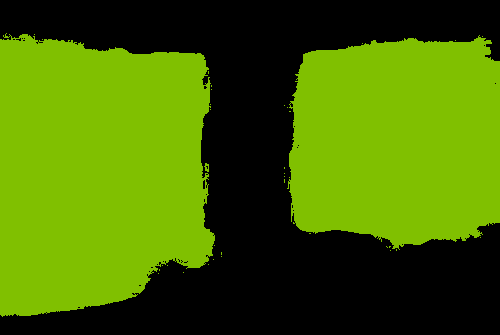
\includegraphics[height=0.11\linewidth]{fig/val_crf_vis/strongweak/2007_000042.png} &
    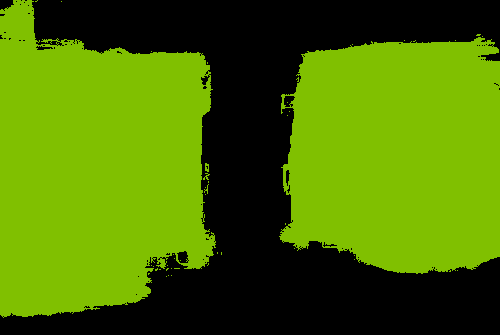
\includegraphics[height=0.11\linewidth]{fig/val_crf_vis/cocomix/2007_000042.png} \\
    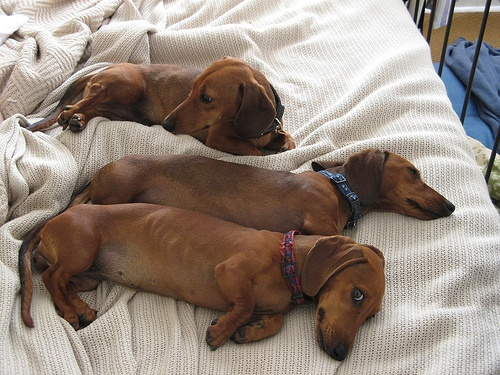
\includegraphics[height=0.122\linewidth]{fig/val_crf_vis/img/2007_002852.jpg} &
    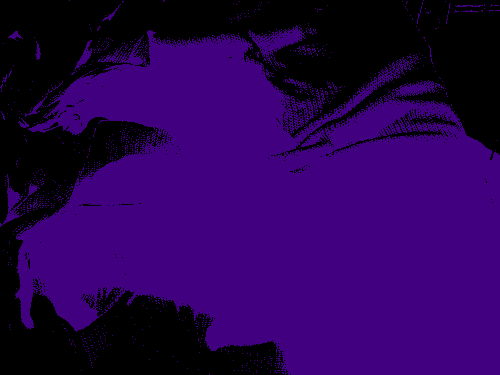
\includegraphics[height=0.122\linewidth]{fig/val_crf_vis/adaweak/2007_002852.png} &
    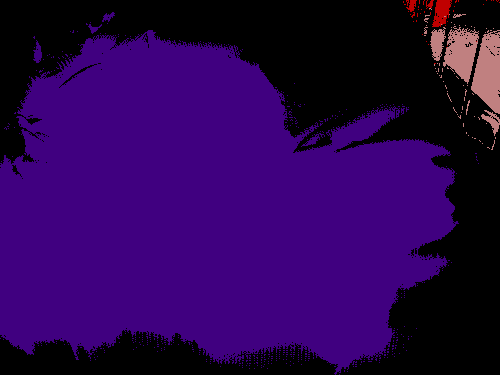
\includegraphics[height=0.122\linewidth]{fig/val_crf_vis/bbox/2007_002852.png} &
    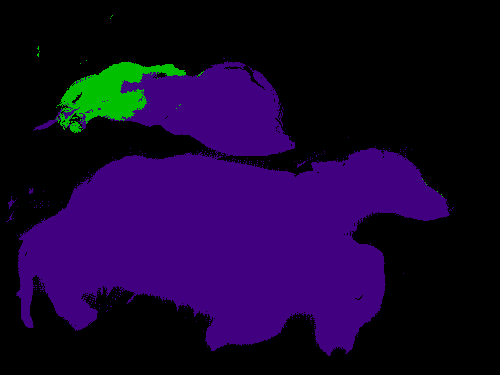
\includegraphics[height=0.122\linewidth]{fig/val_crf_vis/bbox_crf/2007_002852.png} &
    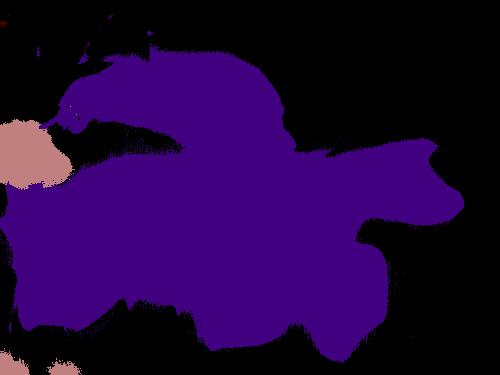
\includegraphics[height=0.122\linewidth]{fig/val_crf_vis/strongweak/2007_002852.png} &
    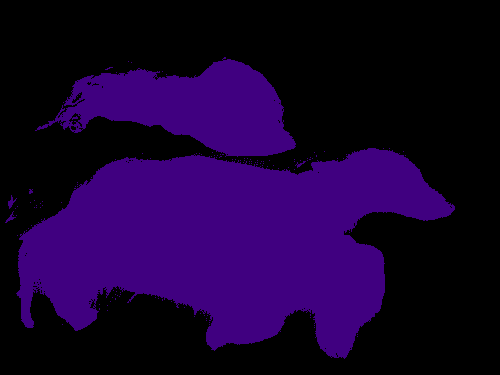
\includegraphics[height=0.122\linewidth]{fig/val_crf_vis/cocomix/2007_002852.png} \\
    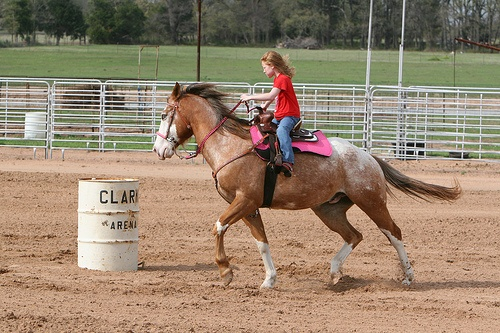
\includegraphics[height=0.11\linewidth]{fig/val_crf_vis/img/2007_003022.jpg} &
    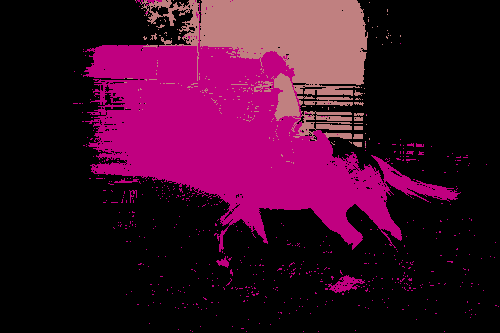
\includegraphics[height=0.11\linewidth]{fig/val_crf_vis/adaweak/2007_003022.png} &
    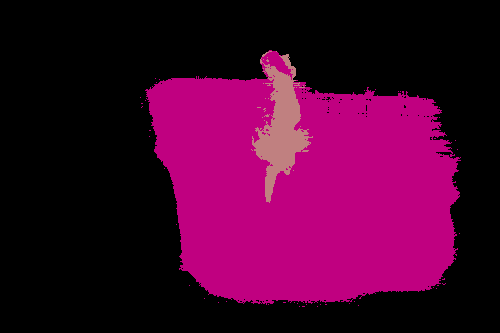
\includegraphics[height=0.11\linewidth]{fig/val_crf_vis/bbox/2007_003022.png} &
    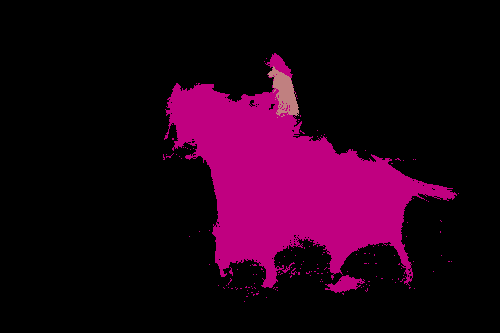
\includegraphics[height=0.11\linewidth]{fig/val_crf_vis/bbox_crf/2007_003022.png} &
    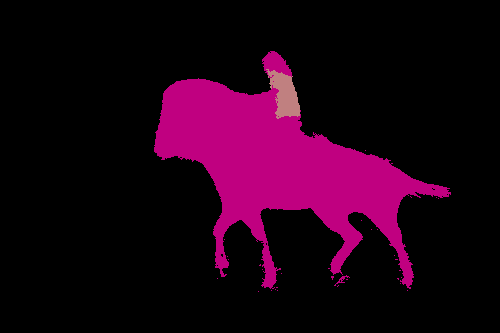
\includegraphics[height=0.11\linewidth]{fig/val_crf_vis/strongweak/2007_003022.png} &
    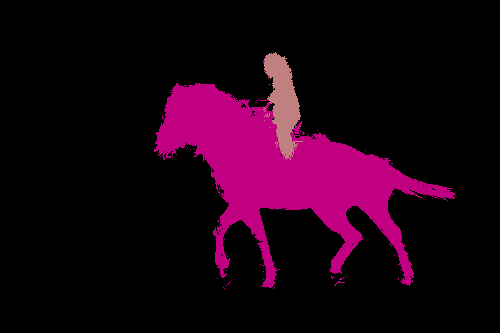
\includegraphics[height=0.11\linewidth]{fig/val_crf_vis/cocomix/2007_003022.png} \\
    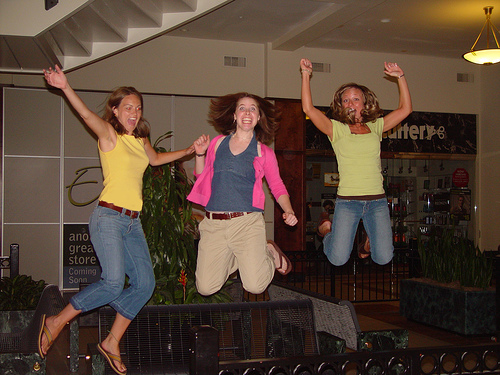
\includegraphics[height=0.123\linewidth]{fig/val_crf_vis/img/2008_003546.jpg} &
    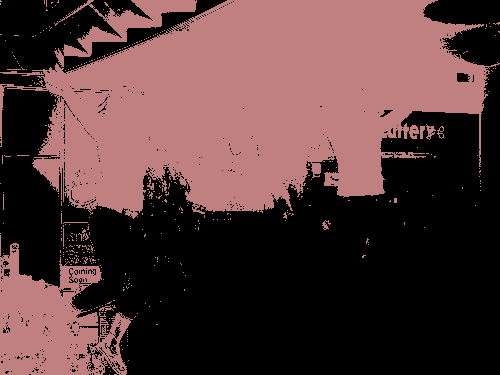
\includegraphics[height=0.123\linewidth]{fig/val_crf_vis/adaweak/2008_003546.png} &
    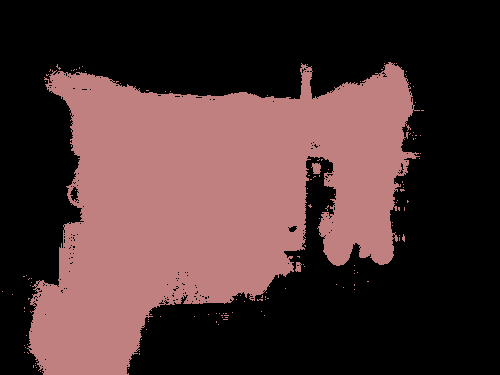
\includegraphics[height=0.123\linewidth]{fig/val_crf_vis/bbox/2008_003546.png} &
    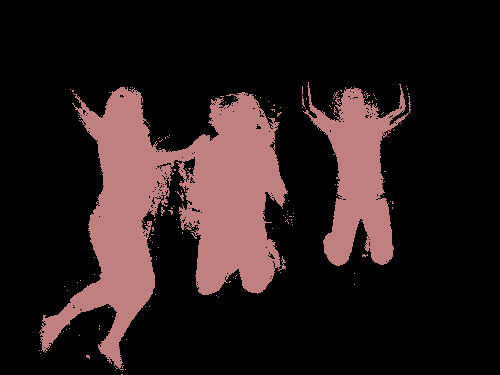
\includegraphics[height=0.123\linewidth]{fig/val_crf_vis/bbox_crf/2008_003546.png} &
    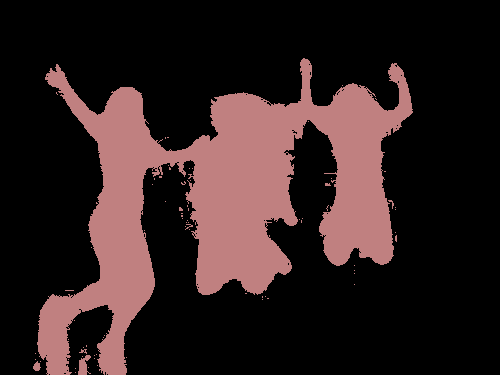
\includegraphics[height=0.123\linewidth]{fig/val_crf_vis/strongweak/2008_003546.png} &
    
\includegraphics[height=0.123\linewidth]{fig/val_crf_vis/cocomix/2008_003546.png} \\
    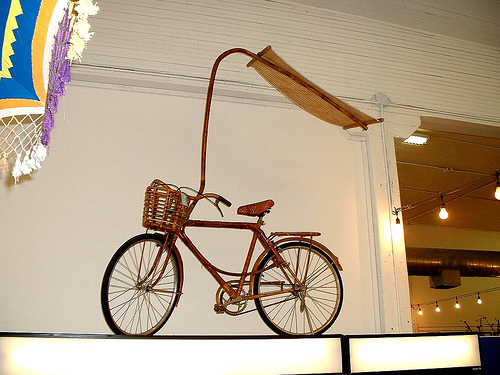
\includegraphics[height=0.123\linewidth]{fig/val_crf_vis/img/2008_004363.jpg} &
    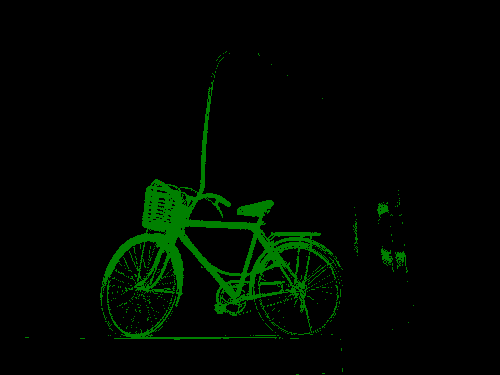
\includegraphics[height=0.123\linewidth]{fig/val_crf_vis/adaweak/2008_004363.png} &
    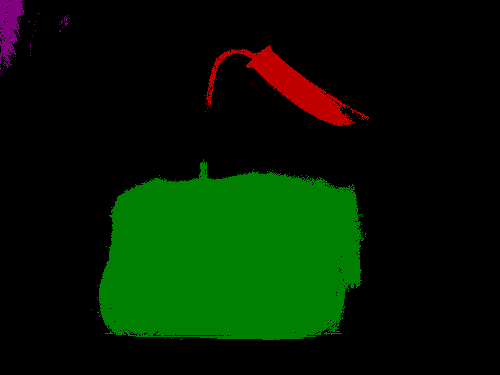
\includegraphics[height=0.123\linewidth]{fig/val_crf_vis/bbox/2008_004363.png} &
    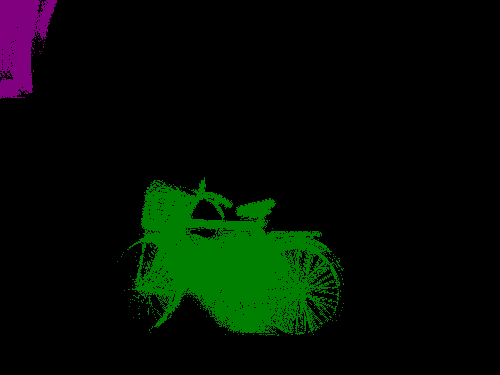
\includegraphics[height=0.123\linewidth]{fig/val_crf_vis/bbox_crf/2008_004363.png} &
    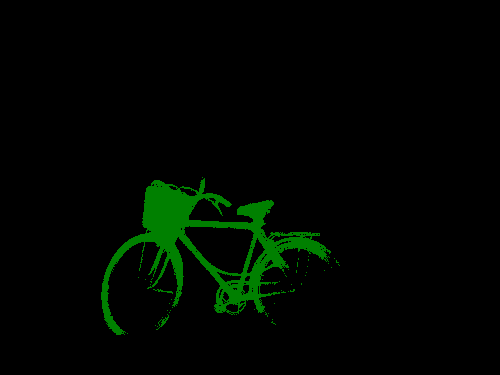
\includegraphics[height=0.123\linewidth]{fig/val_crf_vis/strongweak/2008_004363.png} &
    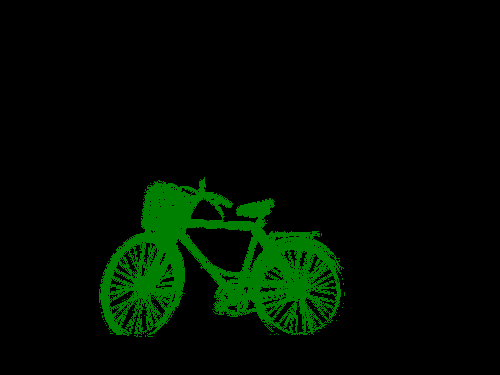
\includegraphics[height=0.123\linewidth]{fig/val_crf_vis/cocomix/2008_004363.png} \\
    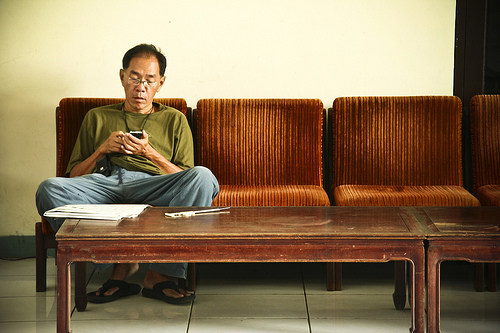
\includegraphics[height=0.11\linewidth]{fig/val_crf_vis/img/2009_001299.jpg} &
    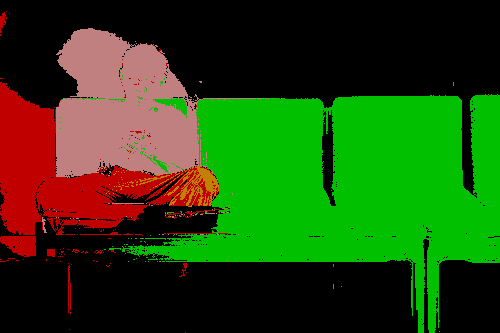
\includegraphics[height=0.11\linewidth]{fig/val_crf_vis/adaweak/2009_001299.png} &
    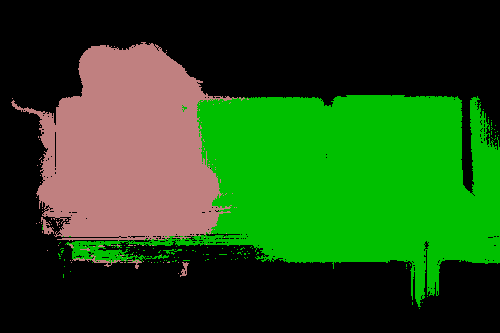
\includegraphics[height=0.11\linewidth]{fig/val_crf_vis/bbox/2009_001299.png} &
    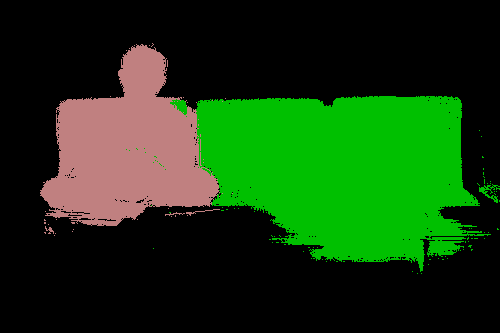
\includegraphics[height=0.11\linewidth]{fig/val_crf_vis/bbox_crf/2009_001299.png} &
    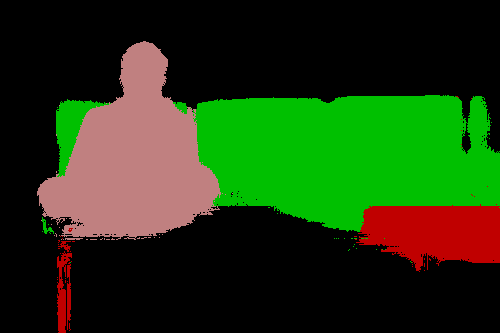
\includegraphics[height=0.11\linewidth]{fig/val_crf_vis/strongweak/2009_001299.png} &
    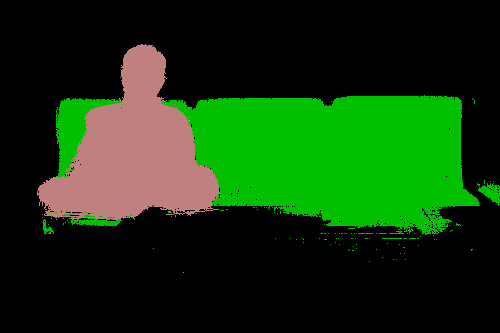
\includegraphics[height=0.11\linewidth]{fig/val_crf_vis/cocomix/2009_001299.png} \\
    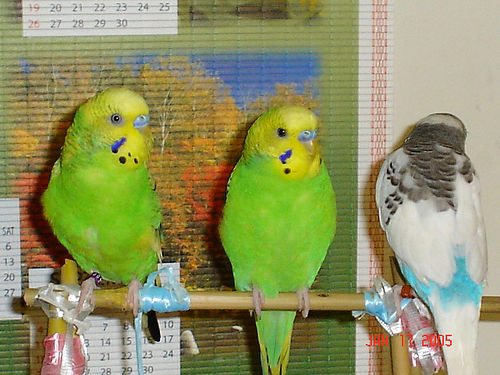
\includegraphics[height=0.123\linewidth]{fig/val_crf_vis/img/2010_004994.jpg} &
    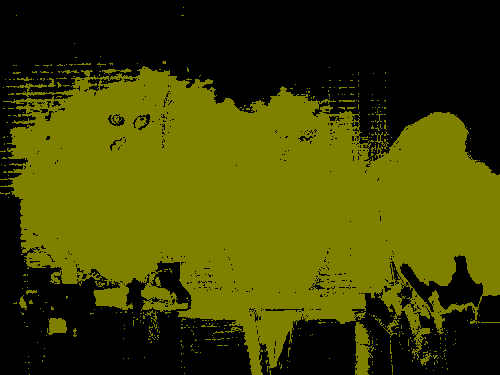
\includegraphics[height=0.123\linewidth]{fig/val_crf_vis/adaweak/2010_004994.png} &
    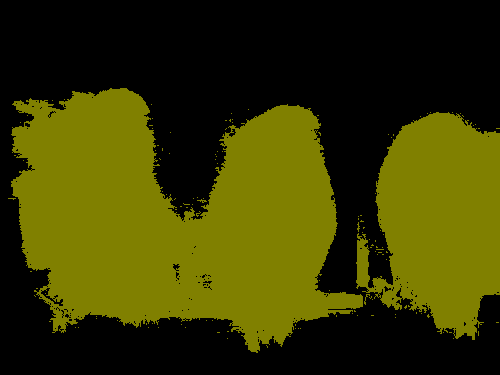
\includegraphics[height=0.123\linewidth]{fig/val_crf_vis/bbox/2010_004994.png} &
    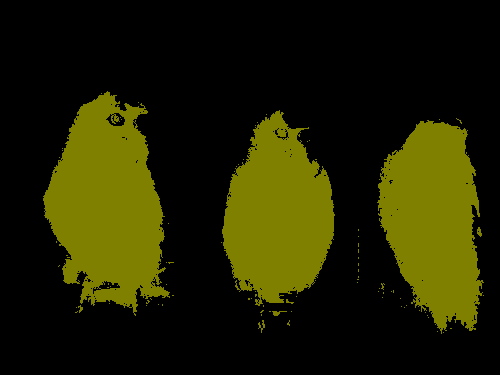
\includegraphics[height=0.123\linewidth]{fig/val_crf_vis/bbox_crf/2010_004994.png} &
    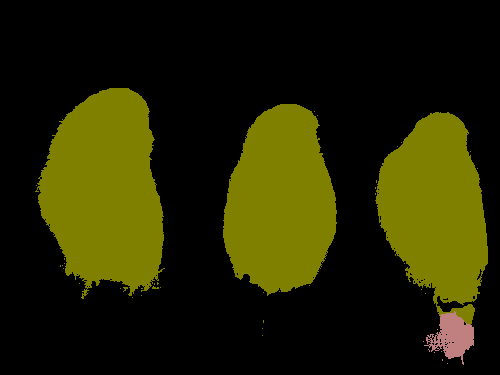
\includegraphics[height=0.123\linewidth]{fig/val_crf_vis/strongweak/2010_004994.png} &
    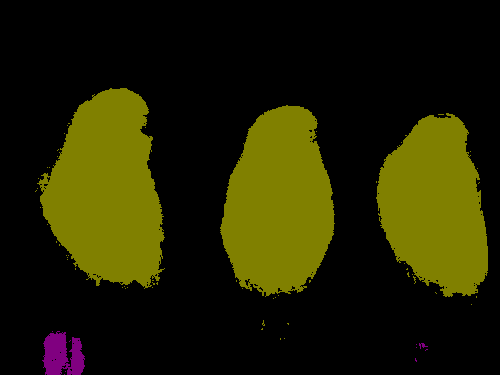
\includegraphics[height=0.123\linewidth]{fig/val_crf_vis/cocomix/2010_004994.png} \\
    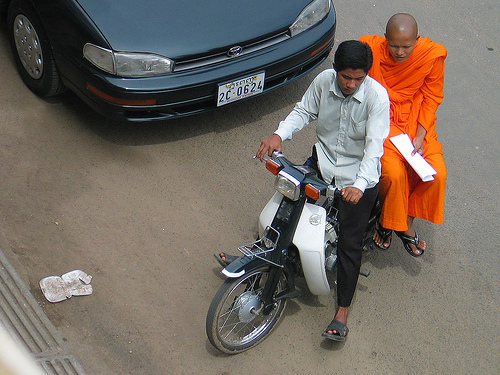
\includegraphics[height=0.122\linewidth]{fig/val_crf_vis/img/2011_002322.jpg} &
    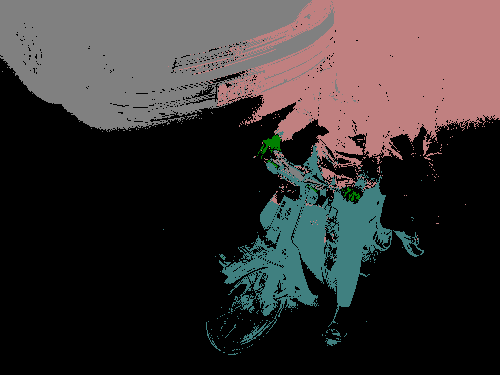
\includegraphics[height=0.122\linewidth]{fig/val_crf_vis/adaweak/2011_002322.png} &
    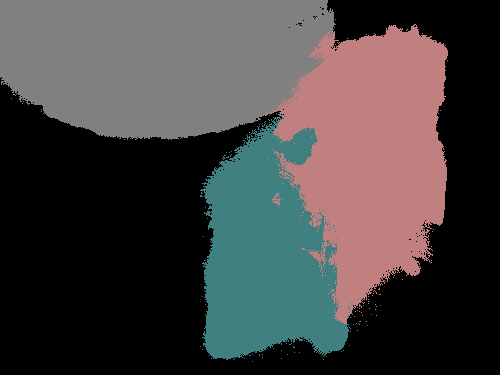
\includegraphics[height=0.122\linewidth]{fig/val_crf_vis/bbox/2011_002322.png} &
    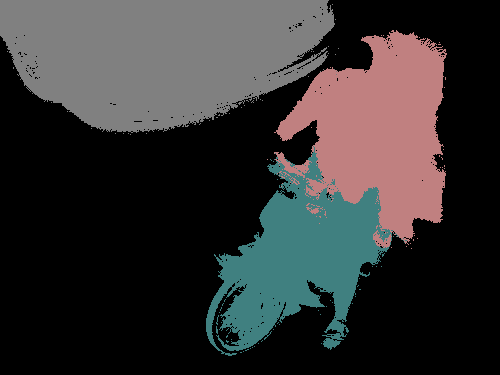
\includegraphics[height=0.122\linewidth]{fig/val_crf_vis/bbox_crf/2011_002322.png} &
    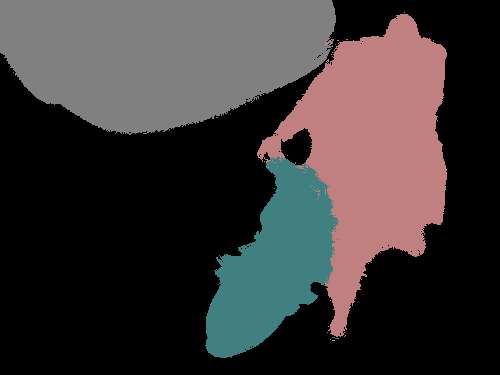
\includegraphics[height=0.122\linewidth]{fig/val_crf_vis/strongweak/2011_002322.png} &
    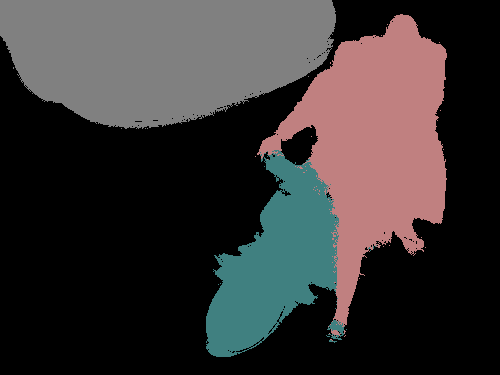
\includegraphics[height=0.122\linewidth]{fig/val_crf_vis/cocomix/2011_002322.png} \\
    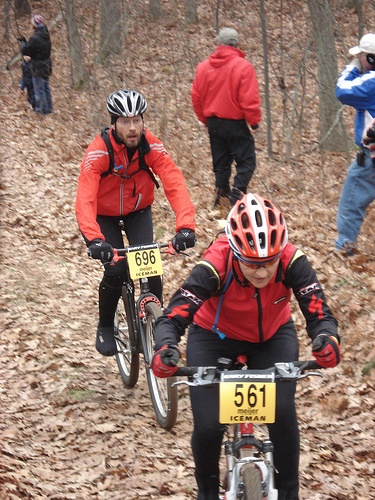
\includegraphics[height=0.13\linewidth]{fig/val_crf_vis/img/2007_001630.jpg} &
    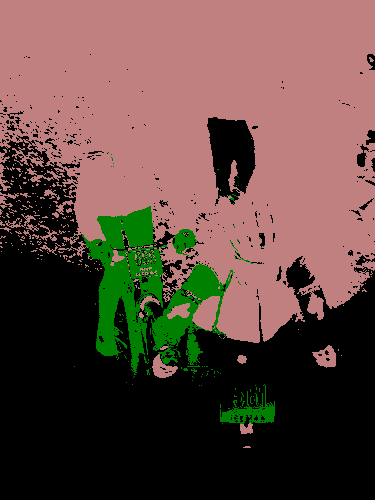
\includegraphics[height=0.13\linewidth]{fig/val_crf_vis/adaweak/2007_001630.png} &
    \includegraphics[height=0.13\linewidth]{fig/val_crf_vis/bbox/2007_001630.png} &
    \includegraphics[height=0.13\linewidth]{fig/val_crf_vis/bbox_crf/2007_001630.png} &
    \includegraphics[height=0.13\linewidth]{fig/val_crf_vis/strongweak/2007_001630.png} &
    \includegraphics[height=0.13\linewidth]{fig/val_crf_vis/cocomix/2007_001630.png} \\
    \includegraphics[height=0.15\linewidth]{fig/val_crf_vis/img/2007_005331.jpg} &
    \includegraphics[height=0.15\linewidth]{fig/val_crf_vis/adaweak/2007_005331.png} &
    \includegraphics[height=0.15\linewidth]{fig/val_crf_vis/bbox/2007_005331.png} &
    \includegraphics[height=0.15\linewidth]{fig/val_crf_vis/bbox_crf/2007_005331.png} &
    \includegraphics[height=0.15\linewidth]{fig/val_crf_vis/strongweak/2007_005331.png} &
    \includegraphics[height=0.15\linewidth]{fig/val_crf_vis/cocomix/2007_005331.png} \\
\hline \hline
    \includegraphics[height=0.11\linewidth]{fig/val_crf_vis/img/2007_000830.jpg} &
    \includegraphics[height=0.11\linewidth]{fig/val_crf_vis/adaweak/2007_000830.png} &
    \includegraphics[height=0.11\linewidth]{fig/val_crf_vis/bbox/2007_000830.png} &
    \includegraphics[height=0.11\linewidth]{fig/val_crf_vis/bbox_crf/2007_000830.png} &
    \includegraphics[height=0.11\linewidth]{fig/val_crf_vis/strongweak/2007_000830.png} &
    \includegraphics[height=0.11\linewidth]{fig/val_crf_vis/cocomix/2007_000830.png} \\
    \includegraphics[height=0.11\linewidth]{fig/val_crf_vis/img/2007_001175.jpg} &
    \includegraphics[height=0.11\linewidth]{fig/val_crf_vis/adaweak/2007_001175.png} &
    \includegraphics[height=0.11\linewidth]{fig/val_crf_vis/bbox/2007_001175.png} &
    \includegraphics[height=0.11\linewidth]{fig/val_crf_vis/bbox_crf/2007_001175.png} &
    \includegraphics[height=0.11\linewidth]{fig/val_crf_vis/strongweak/2007_001175.png} &
    \includegraphics[height=0.11\linewidth]{fig/val_crf_vis/cocomix/2007_001175.png} \\
    {\footnotesize Image} & {\footnotesize Weak-EM-Adapt} & {\footnotesize
      Weak-Bbox-Baseline} & {\footnotesize Weak-Bbox-Seg} & {\footnotesize
      Semi (1,464 Strong)} & {\footnotesize Strong-Cross-Joint} \\
  \end{tabular}
  }
  %\vspace{-0.3cm}
  \caption{Qualitative DeepLab-CRF segmentation results on the PASCAL
    VOC 2012 \textsl{val} set with the proposed training methods (see
    \secref{sec:test_qualitative} for details). We show difficult
    examples in the last two rows.}
  \label{fig:ValResults}
\end{figure*}

\subsection{Evaluation on PASCAL VOC 2012 Test Set and Comparison with State-of-Art}

We report in \tabref{tab:voc2012} our DeepLab-CRF results on the
PASCAL VOC 2012 \textsl{test} set, evaluating the performance of the
proposed training methods on the official segmentation benchmark. We
also compare our results with other leading models from the PASCAL
leaderboard, namely \textsl{Hypercolumn-SDS}
\citep{hariharan2014hypercolumns}, \textsl{MSRA-CFM}
\citep{dai2014convolutional}, \textsl{FCN-8s} \citep{long2014fully},
and \textsl{TTI-Zoomout-16} \citep{mostajabi2014feedforward}.

The \textsl{DeepLab-CRF} model \citep{chen2014semantic} trained with
all PASCAL \textsl{trainval\_aug} strong pixel-level annotations is
the current state-of-art with 66.4\% IOU performance, which we aim to
reach with weaker annotation during training. Using only the weak
image-level PASCAL \textsl{trainval\_aug} labels, the proposed
\textsl{Weak-EM-Adapt} method yields only 39.0\%. When we have access
to weak bounding box annotation, we can do much better, achieving
54.2\% with \textsl{Weak-Bbox-Baseline} and 60.4\% with
\textsl{Weak-Bbox-Seg}, only 6\% worse than the target
performance. We perform even better when we only have access to a
small subset of pixel-level annotated images and use just the
image-level annotations of the remaining \textsl{trainval\_aug}
images in the semi-supervised learning setting: 63.5\% with 1,464
strong annotations and 66.4\% with 2,913 strong
annotations. Remarkably, in this last \textsl{Semi (2,913)} experiment
we exactly match the performance of the model trained with all
strongly annotated images.

We achieve our best result in the cross-dataset training scenario,
using all available PASCAL and MS-COCO pixel-level annotations. This
\textsl{Strong-Cross-Joint} result sets the new state-of-art on the
official PASCAL VOC 2012 benchmark with 70.4\% IOU, outperforming all
previous publicly reported results by more than 3\%.

\begin{table*}[htb!]\scriptsize
 \caption{Benchmark IOU (\%) results on PASCAL VOC 2012
   \textsl{test}. Links to the PASCAL evaluation server are 
   included in the PDF.}
\setlength{\tabcolsep}{3pt}
%\hspace{-1.8cm}
\resizebox{2.1\columnwidth}{!}{
\begin{tabular}{|l||c*{20}{|c}||c|}
\hline 
Method          & bkg &  aero & bike & bird & boat & bottle& bus & car  &  cat & chair& cow  &table & dog  & horse & mbike& person& plant&sheep& sofa &train & tv   & mean \\
\hline \hline
%% Idiap-base+ILP+sppxl      & 74.7 & 38.8 & 19.8 & 27.5 & 21.7 & 32.8 & 40.0 & 50.1 & 47.1 & 7.2 & 44.8 & 15.8 & 49.4 & 47.3 & 36.6 & 36.4 & 24.3 & 44.5 & 21.0 & 31.5 & 41.3 & 35.8 \\
%% Idiap-base+ILP+seg        & 78.7 & 48.0 & 21.2 & 31.1 & 28.4 & 35.1 & 51.4 & 55.5 & 52.8 & 7.8 & 56.2 & 19.9 & 53.8 & 50.3 & 40.0 & 38.6 & 27.8 & 51.8 & 24.7 & 33.3 & 46.3 & 40.6 \\
%% \hline \hline
Hypercolumn-SDS & 88.9 & 68.4 & 27.2 & 68.2 & 47.6 & 61.7 & 76.9 & 72.1 & 71.1 & 24.3 & 59.3 & 44.8 & 62.7 & 59.4 & 73.5 & 70.6 & 52.1 & 63.0 & 38.1 & 60.0 & 54.1 & 59.2 \\   
MSRA-CFM        & -    & 75.7 & 26.7 & 69.5 & 48.8 & 65.6 & 81.0 & 69.2 & 73.3 & 30.0 & 68.7 & 51.5 & 69.1 & 68.1 & 71.7 & 67.5 & 50.4 & 66.5 & 44.4 & 58.9 & 53.5 & 61.8 \\
FCN-8s          & -    & 76.8 & 34.2 & 68.9 & 49.4 & 60.3 & 75.3 & 74.7 & 77.6 & 21.4 & 62.5 & 46.8 & 71.8 & 63.9 & 76.5 & 73.9 & 45.2 & 72.4 & 37.4 & 70.9 & 55.1 & 62.2 \\
TTI-Zoomout-16  & 89.8 & 81.9 & 35.1 & 78.2 & 57.4 & 56.5 & 80.5 & 74.0 & 79.8 & 22.4 & 69.6 & 53.7 & 74.0 & 76.0 & 76.6 & 68.8 & 44.3 & 70.2 & 40.2 & 68.9 & 55.3 & 64.4 \\
DeepLab-CRF     & 92.1 & 78.4 & 33.1 & 78.2 & 55.6 & 65.3 & 81.3 & 75.5 & 78.6 & 25.3 & 69.2 & 52.7 & 75.2 & 69.0 & 79.1 & 77.6 & 54.7 & 78.3 & 45.1 & 73.3 & 56.2 & 66.4 \\ 
\hline \hline
\href{http://host.robots.ox.ac.uk:8080/anonymous/6PBVWD.html}{Weak-EM-Adapt}
                & 76.4 & 37.0 & 17.6 & 38.2 & 26.6 & 37.1 & 51.9 & 43.3 & 48.1 & 16.8 & 44.6 & 27.9 & 46.5 & 46.2 & 46.6 & 30.3 & 28.9 & 42.0 & 30.0 & 43.8 & 39.3 & 39.0 \\
\href{http://host.robots.ox.ac.uk:8080/anonymous/UKB05Q.html}{Weak-Bbox-Baseline}
                & 82.9 & 43.6 & 22.5 & 50.5 & 45.0 & 62.5 & 76.0 & 66.5 & 61.2 & 25.3 & 55.8 & 52.1 & 56.6 & 48.1 & 60.1 & 58.2 & 49.5 & 58.3 & 40.7 & 62.3 & 61.1 & 54.2 \\
\href{http://host.robots.ox.ac.uk:8080/anonymous/TKOAVB.html}{Weak-Bbox-Seg}
                & 89.9 & 69.3 & 28.2 & 71.9 & 43.4 & 59.7 & 74.3 & 69.0 & 76.7 & 23.5 & 64.6 & 47.1 & 71.0 & 64.0 & 72.8 & 72.4 & 50.4 & 72.0 & 40.2 & 63.4 & 44.5 & 60.4 \\
\href{http://host.robots.ox.ac.uk:8080/anonymous/IBKVAA.html}{Semi (1,464 strong)}
                & 91.4 & 77.3 & 38.2 & 73.9 & 47.6 & 57.9 & 80.0 & 76.4 & 74.7 & 22.8 & 70.0 & 42.0 & 70.9 & 71.9 & 79.1 & 70.7 & 47.8 & 77.1 & 36.1 & 68.1 & 59.8 & 63.5 \\
\href{http://host.robots.ox.ac.uk:8080/anonymous/VUCMQV.html}{Semi (2,913 strong)}
                & 92.3 & 81.3 & {\bf 43.8} & 78.3 & 50.2 & 60.4 & 81.2 & 77.5 & 77.5 & 26.8 & 70.8 & 47.0 & 74.8 & 73.0 & 80.8 & 76.0 & 50.8 & 78.0 & 39.7 & 72.9 & 60.9 & 66.4 \\
\hline
\href{http://host.robots.ox.ac.uk:8080/anonymous/L3SZRO.html}{Strong-Cross-Joint}
                & {\bf 93.2} & {\bf 85.3} & 36.2 & {\bf 84.8} & {\bf 61.2} & {\bf 67.5} & {\bf 84.7} & {\bf 81.4} & {\bf 81.0} & {\bf 30.8} & {\bf 73.8} & {\bf 53.8} & {\bf 77.5} & {\bf 76.5} & {\bf 82.3} & {\bf 81.6} & {\bf 56.3} & {\bf 78.9} & {\bf 52.3} & {\bf 76.6} & {\bf 63.3} & {\bf 70.4} \\
\hline
 \end{tabular}
} 
\label{tab:voc2012}
\end{table*}

 %%% Local Variables:
 %%% mode: latex
 %%% TeX-master: "top.tex"
 %%% End:
